\documentclass[journal]{IEEEtran}

\usepackage{amsmath,amsfonts,amssymb,bm}
\usepackage{amsthm}
\usepackage{graphicx}
\usepackage{booktabs,array,multirow}
\usepackage{cite}
\usepackage{url}
\usepackage{textcomp}
\usepackage{stfloats}
\usepackage{algorithm,algorithmic}
\usepackage[hidelinks]{hyperref}
\usepackage{microtype}

\newtheorem{theorem}{Theorem}[section]
\newtheorem{corollary}[theorem]{Corollary}
\newtheorem{proposition}[theorem]{Proposition}
\newtheorem{assumption}[theorem]{Assumption}
\newtheorem{remark}[theorem]{Remark}

\hyphenation{op-tical net-works semi-conduc-tor PAC-Bayesian Takagi--Sugeno}

\begin{document}

\title{An Auditable Complexity-Aware PAC-Bayesian Framework for Linear and Takagi--Sugeno Time-Series Forecasting under Temporal Dependence}

\author{Muneef Abdulkareem Farea Ahmed%
\thanks{M. A. F. Ahmed is with the Faculty of Computer and Information Technology, Sana'a University, Sana'a, Yemen (e-mail: muneef.ahmed@su.edu.ye).}}

\markboth{Manuscript under review}%
{Ahmed: Complexity-Aware PAC-Bayesian Certificates for TSK Forecasting}

\maketitle

\begin{abstract}
PAC-Bayesian certificates for time-series predictors can be formally valid yet operationally uninformative if the prior reuses certification data, the loss is unbounded, or structural choices are not charged. We give a computable specialization of a known time-uniform supermartingale PAC-Bayes bound for ridge and first-order Takagi--Sugeno (TSK) forecasters with overlapping, potentially nonstationary forecast windows. A chronological segment constructs every candidate prior, including scaling, fuzzy antecedents, ridge penalty, and diagonal Gaussian localization. A finite hierarchical code explicitly charges model family, lag, ridge penalty, radius, and realized rule count. The guarantee concerns conditional sequential risk for a clipped normalized squared loss; it is not a bound on raw test RMSE.

A development ablation on 30 synthetic series separates structural sparsity from top-three activation sparsity. Relative to a fixed 12-rule TSK model, radius-controlled TSK reduced the randomized dimension by 95.9 coefficients, Gaussian KL by 22.92, and the certificate by 0.0631 on average; its certificate was tighter in 28 of 30 paired series. Top-three activation alone had negligible certificate effect because it did not reduce the randomized dimension. Ridge nevertheless retained the tightest mean certificate. A first energy deployment gate failed on the three-zone Tetouan development data, motivating a stricter gate frozen before an independent four-region PJM study. The frozen decisions improved test RMSE by 49.13--57.97\% and asymmetric cost by 50.30--58.64\% over a seven-day seasonal-naive fallback. Three decisions selected ridge and the fourth a one-rule TSK model, so the confirmatory result supports complexity-aware selection and abstention, not nonlinear fuzzy-model superiority.
\end{abstract}

\begin{IEEEkeywords}
PAC-Bayesian learning, Takagi--Sugeno fuzzy systems, time-series forecasting, martingales, temporal dependence, structural sparsity, risk certificates.
\end{IEEEkeywords}

\section{Introduction}
\label{sec:introduction}

Time-series predictors are commonly selected by validation error and assessed on a held-out horizon. This workflow measures empirical forecasting performance, but it does not by itself quantify the conditional risk of a data-dependent model when lagged examples overlap, the observations are temporally dependent, and the underlying process may change over time. The limitation is especially relevant for flexible forecasting systems whose complexity depends on several jointly selected structural and numerical choices.

Takagi--Sugeno (TSK) systems represent nonlinear dynamics through convex combinations of local affine rules. Their behavior depends on the lag order, antecedent geometry, number of rules, and regularization of the consequent parameters. These choices affect accuracy, interpretability, and effective statistical complexity. In many forecasting studies, however, the rule count and consequent dimension are treated as implementation details rather than explicit components of a generalization certificate.

PAC-Bayesian analysis provides a natural language for relating empirical loss to a prior--posterior complexity term. In sequential forecasting, a certificate can nevertheless be misleading if the prior is localized with certification observations, squared loss is treated as bounded without justification, or lag, regularization, radius, and rule-count choices are selected without paying their complexity cost. Moreover, a non-vacuous certificate need not identify the predictor with the lowest raw test RMSE or the best operational cost.

This study develops an auditable computational framework for linear and first-order TSK forecasting under overlapping and potentially nonstationary windows. The time-uniform supermartingale argument used in the analysis is established in the PAC-Bayes literature and is not presented as a new concentration theorem. The methodological contribution lies in the chronological construction of the candidate priors, explicit hierarchical charging of the complete model index, analytic evaluation of a Gaussian empirical-risk upper bound, separation of structural sparsity from activation sparsity, and integration of the certificate into a frozen model-selection and abstention protocol.

The central claim is deliberately limited. We do not introduce a new fuzzy clustering algorithm, prove that radius-based rule construction dominates all fixed rule bases, or show that TSK models universally outperform linear and seasonal predictors. Instead, we ask whether complete removal of rule blocks makes TSK complexity auditable and whether a valid certificate can serve as one conservative screening component inside a broader deployment rule.

The contributions are as follows.
\begin{itemize}
    \item We define a chronological candidate family with complete structural index $M=(F,p,\gamma,r,K)$, where $F$ denotes the model family, $p$ the lag, $\gamma$ the ridge penalty, $r$ an optional radius, and $K$ the realized rule count. Scaling, antecedent geometry, prior means, and prior variances are constructed only from the initial segment.
    \item We provide a computable bounded-loss specialization of the established time-uniform supermartingale PAC-Bayes framework \cite{chugg2023unified}. The contribution is the measurable linear/TSK specialization, augmented hierarchical prior, analytic empirical-risk upper bound, and audited implementation.
    \item We distinguish structural rule-count reduction from sparse activation. A synthetic development study compares ridge, fixed-$K$ TSK, radius-controlled all-active TSK, and radius-controlled Top-3 TSK. A subsequent sensitivity analysis over $K\in\{2,3,4,6,8,12\}$ separates the effect of reducing rule count from any additional benefit of radius construction.
    \item We expose actual posterior-center fuzzy rules from a multi-rule SETAR model and from the Tetouan development model. These examples support inspection of the learned local structures without treating them as physical truth or as directly certified deterministic predictors.
    \item We report a negative Tetouan development gate and an internally locked PJM holdout evaluation. Secondary SARIMA and exponential-smoothing benchmarks are explicitly labeled post hoc because they were designed after the PJM outcomes were opened and do not modify the frozen gate or its original claim.
\end{itemize}

The evidence supports an integration claim rather than a fuzzy-model superiority claim. Structural rule reduction substantially lowers dimension, KL, and certificate value relative to an unnecessarily dense 12-rule TSK model. Small fixed rule bases can, however, match or tighten the radius-controlled certificate, and ridge remains the easiest family to certify on average. The independent energy decisions mostly select linear predictors, while the secondary statistical baselines show that stronger forecasting alternatives can improve further on the deployed models. The certificate therefore functions as an auditable risk-screening quantity, not as a direct guarantee of raw RMSE, future stability, or model-class dominance.

The remainder of the paper reviews the relevant literature, defines the chronological model family and the three prediction objects used in the study, formalizes the augmented hierarchical prior, describes the development and operational protocols, and reports the structural, interpretability, and decision results.

\section{Related Work and Positioning}
\label{sec:related_work}

\subsection{PAC-Bayes under Dependence and Sequential Observation}
PAC-Bayes for dependent observations is established. Chromatic and blocking arguments cover dependency graphs and stationary mixing processes \cite{ralaivola2010chromatic}; oracle inequalities have been developed for weakly dependent time-series prediction \cite{alquier2012model,alquier2013prediction}; and recent results address Markov models and stable nonlinear dynamical systems \cite{banerjee2021tempered,eringis2024dynamical}. These approaches typically require explicit dependence, stationarity, boundedness, or stability assumptions.

Martingale and supermartingale methods provide a different route. Seldin \emph{et al.} derived PAC-Bayesian inequalities for martingales \cite{seldin2012martingales}. Online and time-uniform constructions subsequently allowed data-dependent posterior sequences while keeping the prior predictable \cite{haddouche2022online,chugg2023unified}. We use this route because overlapping lag windows form an adapted sequence, and because it avoids treating an estimated mixing coefficient as known. The bounded-loss formula used here is a direct specialization of this literature, not a new general concentration inequality.

\subsection{Computable and Non-Vacuous Certificates}
A formal inequality becomes useful only when the prior, posterior, and empirical term can be computed without hidden data reuse. Data-dependent priors can be valid when their information source is explicitly separated or otherwise controlled \cite{parrado2012dataprior,rivasplata2020beyond}. Work on neural-network certificates shows that prior localization and posterior-scale selection are decisive for tightness \cite{perezortiz2021tighter}. Foong \emph{et al.} show that small-sample PAC-Bayes bounds may remain looser than direct test bounds even after careful optimization \cite{foong2021small}. Heavy-tail and unbounded-loss PAC-Bayes results offer alternatives to clipping \cite{haddouche2021unleashed,haddouche2023heavy,rodriguez2024more}; the current implementation does not claim those guarantees and instead reports clipping explicitly.

\subsection{Sparse TSK Systems}
Bayesian TSK models, block-sparse dynamic fuzzy models, and sparse rule or coefficient learning are well developed \cite{gu2018btsk,li2018blocksparse,li2022bayesiants,lughofer2010sparsefis,luo2013hierarchical,wiktorowicz2022timeseries}. Clustering-based rule construction and online TSK identification are also classical \cite{Chiu1994Cluster,angelov2004online}. Existing work generally targets prediction, parameter estimation, or interpretability; it does not provide the specific audited chain from a prior-only radius cover to a realized randomized dimension, KL cost, and sequential certificate.

\begin{table*}[t]
\centering
\caption{Positioning relative to representative PAC-Bayes literature. ``This work'' uses a known time-uniform supermartingale route; its contribution is the chronological, computable specialization and the structural/operational evaluation.}
\label{tab:prior_work}
\small
\setlength{\tabcolsep}{4pt}
\begin{tabular}{p{2.5cm}p{2.2cm}p{2.4cm}p{3.0cm}p{5.4cm}}
\toprule
Work & Data regime & Loss / guarantee & Main computational focus & Difference from the present study \\
\midrule
Seldin et al. \cite{seldin2012martingales} & Martingales & PAC-Bayes martingale inequalities & General concentration & Provides foundational martingale PAC-Bayes inequalities; no chronological TSK construction or rule-count audit. \\
Chugg et al. \cite{chugg2023unified} & Sequential, non-IID & Time-uniform PAC-Bayes recipes & General supermartingale framework & The bound used here is a bounded-loss specialization, not a competing general theorem. \\
P\'erez-Ortiz et al. \cite{perezortiz2021tighter} & IID classification & Tight neural-network risk certificates & Joint prior/posterior optimization & Motivates computable non-vacuous certificates, but not temporal dependence or fuzzy structure. \\
Foong et al. \cite{foong2021small} & IID, small samples & Tightness limits & Bound-vs-test comparison & Motivates reporting vacuity and clipping; it does not address sequential dependence. \\
Haddouche--Guedj \cite{haddouche2023heavy} & Sequential/heavy-tailed & Supermartingale bounds for heavy tails & Unbounded-loss control & Offers a route beyond clipping; the current implementation deliberately uses bounded clipped loss. \\
Alquier--Wintenberger \cite{alquier2012model} and Eringis et al. \cite{eringis2024dynamical} & Weakly dependent time series / stable systems & Generalization under dependence & Rates or stability/mixing conditions & These require dependence or stability assumptions; the primary certificate here uses predictability and bounded loss instead. \\
This work & Overlapping, possibly nonstationary forecast windows & Conditional sequential clipped risk & Hierarchical structural coding; radius-vs-fixed-$K$ ablation; frozen deployment gate & Empirically separates structural sparsity from activation sparsity and tests a negative development gate followed by an independent confirmatory energy case. \\
\bottomrule
\end{tabular}
\end{table*}


\subsection{Precise Novelty Claim}
The present study does not introduce a new clustering algorithm, a new general PAC-Bayes theorem, or a proof that TSK models dominate linear or seasonal forecasts. Its contribution is the intersection of: (i) a chronologically valid finite prior over complete forecasting structures; (ii) a computable sequential certificate for a linear-in-consequents TSK model; (iii) a controlled fixed-$K$ versus radius-controlled structural ablation; and (iv) an operational protocol that records a negative development case before an independent frozen confirmatory case. Table~\ref{tab:prior_work} makes the distinction from the closest PAC-Bayes literature explicit.

\section{Sequential Setup and Model Family}
\label{sec:model}

\subsection{Chronological Roles}
Let $(\mathcal F_t)_{t\ge0}$ be the data filtration and
\begin{equation}
X_t=(Y_{t-1},\ldots,Y_{t-p})^\top
\label{eq:lag_vector}
\end{equation}
be $\mathcal F_{t-1}$-measurable. Every trajectory is divided, without shuffling, into
$\mathcal D_{\mathrm{prior}}$, $\mathcal D_{\mathrm{bound}}$, $\mathcal D_{\mathrm{validation}}$, and $\mathcal D_{\mathrm{test}}$.
The first segment constructs all candidate-specific priors. The bound segment fits posterior centers, the validation segment selects among the predeclared candidate/posterior family, and the test segment is opened only after selection or deployment decisions are frozen. Certification uses bound plus validation observations; test observations are excluded.

All target scaling parameters are computed from $\mathcal D_{\mathrm{prior}}$. This makes the standardized lag vector, antecedent geometry, and clipping interval measurable at the start of the certification horizon.

\subsection{Ridge and TSK Predictors}
The ridge family uses the design $\phi_{p}(x)=(1,x^\top)^\top$. A first-order TSK system with $K$ rules uses Gaussian memberships
\begin{align}
\mu_{kj}(x_j)&=\exp\!\left[-\frac{(x_j-c_{kj})^2}{2s_{kj}^2}\right],\\
\alpha_k(x)&=\frac{\prod_j\mu_{kj}(x_j)}{\sum_{\ell=1}^{K}\prod_j\mu_{\ell j}(x_j)},
\label{eq:memberships}
\end{align}
and prediction
\begin{equation}
f_{M,a}(x)=\sum_{k=1}^{K}\alpha_k(x)(a_{k0}+a_k^\top x).
\label{eq:tsk}
\end{equation}
With fixed antecedents, the predictor is linear in the stacked consequent vector $a$. Its design vector is
\begin{equation}
\phi_M(x)=\big[\alpha_1(x)(1,x^\top),\ldots,\alpha_K(x)(1,x^\top)\big]^\top,
\label{eq:design}
\end{equation}
with randomized dimension $D_M=K(p+1)$. Ridge is the $D_M=p+1$ linear family and is kept separate in the structural prior.

\subsection{Prior-Only Antecedent Constructions}
For radius-controlled TSK, standardized prior inputs are covered by deterministic farthest-first centers until all prior points lie within radius $r$ or the predeclared rule cap is reached. Candidates that hit the cap before coverage are ineligible. Rule spreads are estimated from prior assignments with fixed numerical floors and ceilings. The resulting $K=K(r,\mathcal D_{\mathrm{prior}})$ is therefore random before conditioning, but is $\mathcal G_0$-measurable after the prior segment.

The fixed-$K$ baseline uses deterministic farthest-first construction with exactly $K_{\max}$ centers. Radius-controlled all-active TSK retains all rule weights. Radius Top-3 TSK uses the same antecedents but keeps only the three largest firing strengths per sample before renormalization. This latter operation changes computation and occasionally prediction, but not $D_M$; it is therefore an activation-sparsity ablation rather than structural sparsity.

\subsection{Complete Model Index and Ridge Fits}
The discrete model index is
\begin{equation}
M=(F,p,\gamma,r,K),
\label{eq:model_index}
\end{equation}
where $F$ identifies ridge, fixed-$K$ TSK, radius TSK, or the development-only Top-3 family. The radius is absent for ridge and fixed-$K$ candidates. For every predeclared $M$, the prior and posterior centers use the same ridge penalty $\gamma$:
\begin{align}
\mu_{P,M}&=(\Phi_{P,M}^\top\Phi_{P,M}+\gamma I)^{-1}\Phi_{P,M}^\top y_P,\\
\mu_{Q,M}&=(\Phi_{B,M}^\top\Phi_{B,M}+\gamma I)^{-1}\Phi_{B,M}^\top y_B.
\label{eq:centers}
\end{align}
Thus $\gamma$ is not selected silently after the prior is fixed: all candidate-specific prior centers are functions only of the configuration and $\mathcal D_{\mathrm{prior}}$. Computing them lazily in software is mathematically equivalent to constructing the whole finite family at $\mathcal G_0$.

The validation ordering is RMSE, then MAE, consequent dimension, rule count, radius, ridge penalty, and lag. A separate development analysis minimizes the certificate instead of validation RMSE; this is not the primary predictive selection rule.

\subsection{Bounded Certified Loss}
Let
\begin{equation}
B=c_B\max\left\{1,\max_{t\in\mathcal D_{\mathrm{prior}}}|Y_t|\right\},
\label{eq:B}
\end{equation}
where $c_B\ge1$ is fixed before certification. Define $\bar Y_t=\Pi_{[-B,B]}Y_t$ and $\bar f_h(X_t)=\Pi_{[-B,B]}f_h(X_t)$. The certified loss is
\begin{equation}
\ell_t(h)=\frac{(\bar Y_t-\bar f_h(X_t))^2}{4B^2}\in[0,1].
\label{eq:loss}
\end{equation}
Target and forecast clipping rates are reported separately. The operational energy studies use $c_B=1.25$; the synthetic development study uses $c_B=1$.

\section{Computable Sequential PAC-Bayes Certificate}
\label{sec:certificate}

\subsection{Augmented Hierarchical Prior}
Condition on the information $\mathcal G_0$ available after $\mathcal D_{\mathrm{prior}}$. The hypothesis space is augmented with the discrete labels used to construct the Gaussian component:
\begin{equation}
 h=(M,v,s,a),\qquad M=(F,p,\gamma,r,K),
\label{eq:augmented_hypothesis}
\end{equation}
where $v$ denotes the prior-localization variant, $s$ the prior-scale component, and $a$ the consequent vector. The prediction depends on $(M,a)$; the labels $(v,s)$ make the mixture accounting explicit.

Let $\pi_F$, $\pi_p$, and $\pi_\gamma$ be uniform on the predeclared family, lag, and ridge-penalty grids. For ridge and fixed-$K$ families, the radius factor is one; for radius-controlled families, $\pi_{r\mid F}$ is uniform on the radius grid. TSK structures additionally receive the normalized geometric rule-count mass
\begin{equation}
\pi_K(K)=\frac{\exp(-\eta K)}{\sum_{j=1}^{K_{\max}}\exp(-\eta j)},\qquad \eta=\log 2.
\label{eq:kprior}
\end{equation}
The structural mass used by the implementation is therefore
\begin{equation}
\pi(M)=\pi_F(F)\pi_p(p)\pi_\gamma(\gamma)\pi_{r\mid F}(r\mid F)\,\pi_{K\mid F}(K\mid F),
\label{eq:structural_prior}
\end{equation}
where $\pi_{K\mid F}=1$ for ridge and $\pi_{K\mid F}=\pi_K$ for TSK families. For a radius candidate, $K=K(r,\mathcal D_{\mathrm{prior}})$ is fixed after conditioning on $\mathcal G_0$. Ineligible radius candidates receive zero executable mass. For each radius-controlled family,
\begin{equation}
\sum_{r}\pi_{r\mid F}(r\mid F)\pi_K\!\left(K(r)\right)\mathbf 1\{r\text{ eligible}\}\le 1,
\end{equation}
and for any evaluated fixed-$K$ subset, $\sum_{K\in\mathcal K_{\mathrm{exec}}}\pi_K(K)\le1$. The unused family mass is assigned to a dummy hypothesis. Thus the prior is proper without renormalizing after observing which candidates are executable; the reported code lengths are conservative.

For localization variant $v$ and prior scale $s$, let $\omega(v)$ and $\xi(s)$ denote the predeclared mixture masses. The operational studies use a single chronological localized variant, while the development localization ablation uses two equally weighted variants. The scale set is $\mathcal S=\{0.5,1,2,4,8\}$ with uniform mass $\xi(s)=1/5$. For every $(M,v,s)$, define
\begin{equation}
P_{M,v,s}=\mathcal N\!\left(\mu_{P,M,v},\operatorname{diag}(s^2b_{M,v}^2)\right).
\label{eq:prior_gauss}
\end{equation}
The full prior on the augmented space is
\begin{equation}
P(dM,dv,ds,da)=\pi(M)\omega(v)\xi(s)P_{M,v,s}(da),
\label{eq:joint_prior}
\end{equation}
with the remaining structural mass placed on the dummy component.

After observing the certification data, a selected posterior has the form
\begin{equation}
Q=\delta_{\widehat M}\delta_{\widehat v}\delta_{\widehat s}\,
Q_{\widehat M,\widehat v,\widehat s,\widehat\rho},
\label{eq:joint_posterior}
\end{equation}
where
\begin{equation}
Q_{M,v,s,\rho}=\mathcal N\!\left(\mu_{Q,M},\operatorname{diag}(s^2\rho^2b_{M,v}^2)\right),
\label{eq:posterior_gauss}
\end{equation}
and $\rho\in\{0.01,0.03,0.1,0.3,1\}$. Because the component labels are explicit coordinates of the augmented hypothesis, the divergence decomposes exactly as
\begin{align}
\mathrm{KL}(Q\|P)
={}&-\log\pi(\widehat M)-\log\omega(\widehat v)-\log\xi(\widehat s)\nonumber\\
&+\mathrm{KL}\!\left(Q_{\widehat M,\widehat v,\widehat s,\widehat\rho}\middle\|P_{\widehat M,\widehat v,\widehat s}\right).
\label{eq:joint_kl}
\end{align}
The final term is the exact diagonal-Gaussian divergence
\begin{equation}
\frac12\sum_{j=1}^{D_M}\left[
\log\frac{\sigma_{P,j}^2}{\sigma_{Q,j}^2}-1+
\frac{\sigma_{Q,j}^2+(\mu_{Q,j}-\mu_{P,j})^2}{\sigma_{P,j}^2}
\right].
\label{eq:gaussian_kl}
\end{equation}
Selection of $\rho$ needs no additional discrete union penalty because Proposition~\ref{prop:bound} is simultaneous over all $Q\ll P$. Temperature selection is different: it is a choice among concentration inequalities and is charged through the temperature mass $\nu(\lambda)$. The supplementary material gives the proper-mass completion and the componentwise derivation in full.

\subsection{Time-Uniform Bounded-Loss Specialization}
For $h=(M,a)$, write $\mu_t(h)=\mathbb E[\ell_t(h)\mid\mathcal G_{t-1}]$ and
\begin{align}
\widehat R_t(Q)&=\frac1t\sum_{i=1}^{t}\mathbb E_Q[\ell_i],\\
R_t^{\mathrm{seq}}(Q)&=\frac1t\sum_{i=1}^{t}\mathbb E_Q[\mu_i].
\label{eq:risks}
\end{align}

\begin{assumption}[Predictable bounded loss]
For each fixed $h$, the forecast at time $t$ is $\mathcal G_{t-1}$-measurable and $0\le\ell_t(h)\le1$ almost surely.
\end{assumption}

\begin{proposition}[Bounded-loss time-uniform specialization]
\label{prop:bound}
Let $P$ be $\mathcal G_0$-measurable and let $\Lambda$ be a finite positive temperature grid with mass function $\nu$. Conditionally on $\mathcal G_0$, with probability at least $1-\delta$, simultaneously for every $t\ge1$, every $\mathcal G_t$-measurable $Q_t\ll P$, and every $\lambda\in\Lambda$,
\begin{equation}
R_t^{\mathrm{seq}}(Q_t)\le \widehat R_t(Q_t)+\frac{\lambda}{8}+
\frac{\mathrm{KL}(Q_t\|P)+\log[1/(\delta\nu(\lambda))]}{\lambda t}.
\label{eq:main_bound}
\end{equation}
\end{proposition}

Proposition~\ref{prop:bound} is the conditional-Hoeffding instance of the established PAC-Bayes supermartingale recipe \cite{seldin2012martingales,chugg2023unified}. For fixed $h$, $\exp\{\lambda\sum_{i\le t}(\mu_i-\ell_i)-t\lambda^2/8\}$ is a nonnegative supermartingale. Mixing over $P$, applying Ville's inequality, then the Donsker--Varadhan change of measure proves the statement; a union bound charges the finite temperature grid. The proof and the prior-mixture completion are given in the supplementary material.

The reported value is the minimum untruncated right-hand side over the fixed temperature grid, clipped at one only for presentation. Familywise studies allocate $\delta/S$ to each of $S$ predeclared series.

\subsection{Analytic Empirical-Risk Upper Bound}
For fixed antecedents, $f_{M,a}(x)=\phi_M(x)^\top a$ before projection. Therefore
\begin{equation}
\mathbb E_Q[(\bar Y-\phi^\top a)^2]=(\bar Y-\phi^\top\mu_Q)^2+
\phi^\top\operatorname{diag}(\sigma_Q^2)\phi.
\label{eq:secondmoment}
\end{equation}
Projection cannot increase squared distance to $\bar Y\in[-B,B]$. Using the concavity of $u\mapsto\min(1,u)$ gives the pointwise upper bound
\begin{equation}
\widehat r_i(Q)=\min\left\{1,
\frac{(\bar Y_i-\phi_i^\top\mu_Q)^2+
\phi_i^\top\operatorname{diag}(\sigma_Q^2)\phi_i}{4B^2}
\right\}.
\label{eq:empirical_upper}
\end{equation}
The implementation substitutes $t^{-1}\sum_i\widehat r_i(Q)$ for $\widehat R_t(Q)$, which is conservative.

\begin{corollary}[Clipped Bayesian model average]\label{cor:bma}
The clipped Bayesian model-average risk is no larger than the Gibbs risk in Proposition~\ref{prop:bound}, by convexity of squared loss.
\end{corollary}

\subsection{Scope of the Guarantee}
The guarantee is for average conditional risk of the clipped Gibbs predictor, and by convexity its clipped model average, over the observed certification horizon. It is valid for adapted overlapping windows and does not require an estimated mixing coefficient. It is not a guarantee for raw RMSE, an arbitrary deterministic parameter-mean implementation, the future test horizon, or performance relative to a seasonal baseline. Those quantities remain empirical evaluations and are deliberately separated from the certificate.

\section{Experimental Protocol}
\label{sec:experiments}

\subsection{Synthetic Development and Structural Ablation}
The development study uses six processes and five seeds per process, for 30 complete trajectories. Each trajectory retains 2,000 observations after a burn-in of 500 and is split chronologically 20/45/15/20 into prior, bound, validation, and test roles. Table~\ref{tab:synthetic_processes} gives the corrected data-generating definitions.

\begin{table*}[t]
\centering
\caption{Synthetic development processes. Each trajectory retains 2,000 observations after a burn-in of 500.}
\label{tab:synthetic_processes}
\small
\setlength{\tabcolsep}{4pt}
\begin{tabular}{lp{9.5cm}p{4.0cm}}
\toprule
Process & Definition & Purpose \\
\midrule
AR(2) & $Y_t=0.6Y_{t-1}-0.2Y_{t-2}+\varepsilon_t$, $\varepsilon_t\sim\mathcal N(0,0.2^2)$. & Linear short-memory dependence. \\
SETAR & $0.65Y_{t-1}+\varepsilon_t$ if $Y_{t-1}\le0$; otherwise $-0.45Y_{t-1}+0.25Y_{t-2}+\varepsilon_t$. & Threshold nonlinearity. \\
NARMA-10 & Standard tenth-order nonlinear moving-average recursion with $U_t\sim\mathcal U(0,0.5)$. & Nonlinear finite memory. \\
Mackey--Glass & Euler recursion with delay 17 and additive $\mathcal N(0,0.01^2)$ noise. & Delayed nonlinear dynamics. \\
GARCH & Zero-mean GARCH(1,1) with standardized Student-$t_5$ innovations. & Conditional heteroskedasticity and heavy tails. \\
Structural break & AR(1) mean, coefficient, and noise scale change after 60\% of the retained sample. & Deliberate nonstationarity and clipping stress. \\
\bottomrule
\end{tabular}
\end{table*}


The full structural ablation compares four families: ridge; fixed-$K$ all-active TSK with $K=12$; radius-controlled all-active TSK; and radius-controlled Top-3 TSK. Candidate lags are $\{3,5,10,15,20\}$, ridge penalties are $\{10^{-4},10^{-3},10^{-2},10^{-1},1\}$, and radii are $\{0.5,0.75,1,1.25,1.5,1.75,2,2.5,3,4,5\}$. The rule cap is 12. The certificate uses temperatures $\{0.125,0.25,0.5,1,2,4\}$, the prior scales and posterior ratios in Section~\ref{sec:certificate}, and familywise confidence $\delta=0.05/30$.

The original four-family engine evaluated 12,700 eligible candidates with no build failures. Candidate rows contain no test metric. A selected candidate is serialized before its test role is opened. We report both validation-RMSE selection and certificate selection; the former is the primary predictive comparison.

\subsection{Exploratory Fixed-$K$ Sensitivity Extension}
Because comparison with only $K=12$ can mechanically favor any smaller rule base, we added an explicitly exploratory development extension with fixed rule counts $K\in\{2,3,4,6,8,12\}$. The radius-controlled all-active family, lag grid, ridge-penalty grid, prior construction, posterior grids, loss, confidence allocation, and chronological roles were unchanged. Each fixed $K$ pays the same normalized geometric rule-count code as the radius-controlled family; selecting $K$ is therefore not free. The degenerate one-rule case is excluded from the primary fuzzy sensitivity analysis because it reduces to an affine predictor.

For every series and every $K$, candidates are selected independently by validation RMSE and by certificate value before the synthetic test role is opened. Radius-controlled TSK is compared with each fixed $K$ and with the best fixed-$K$ candidate selected from the predeclared grid. Paired differences are summarized using 20,000-resample bootstrap confidence intervals and Wilcoxon signed-rank tests with Holm correction across the six $K$ values. This extension is developmental and postdates the original $K=12$ ablation; it does not modify the frozen PJM gate, decisions, or confirmatory outcomes. The extended engine evaluated 16,450 eligible candidates with no build failures.

\subsection{Tetouan Development Decision Case}
The first operational study uses the UCI Tetouan City power-consumption data \cite{uci_tetouan_849}. Ten-minute observations are aggregated to two-hour means for three zones. Each zone is split 20/45/15/20. The candidate families are ridge, fixed eight-rule TSK, and radius-controlled TSK with lags $\{3,6,12\}$. The initial gate required an untruncated certificate no larger than 0.20, certification clipping no larger than 5\%, and validation RMSE no worse than a 12-step seasonal-naive fallback. Underforecast errors receive weight two and overforecast errors weight one. This study is explicitly developmental: its test outcome is used to redesign, not confirm, the later gate.

\subsection{Independent PJM Confirmatory Case}
After the Tetouan outcome, a stricter gate was frozen before inspecting PJM test outcomes. Four predeclared regional hourly-load series---AEP, COMED, DAYTON, and PJME---are taken from the public Hourly Energy Consumption collection \cite{mulla_hourly_energy}. Duplicate timestamps are averaged; the common interval from 1 January 2012 through 2 August 2018 is aggregated to 2,406 daily means per region, requiring at least 23 hourly values per retained day. No exogenous variables are used.

The chronological split is again 20/45/15/20. The candidate families are ridge, fixed eight-rule TSK, and radius-controlled TSK. Lags are $\{7,14,28\}$ days, radii are $\{0.75,1,1.25,1.5,2,2.5\}$, and ridge penalties are unchanged. Confidence is $0.05/4$.

A candidate is deployment-eligible only if all seven frozen conditions hold:
\begin{enumerate}
    \item untruncated certificate $\le0.10$;
    \item certification target clipping $\le2\%$;
    \item validation RMSE improvement over seven-day seasonal naive $\ge5\%$;
    \item validation asymmetric-cost improvement $\ge5\%$;
    \item nonnegative RMSE improvement in at least three of four chronological validation blocks;
    \item nonnegative cost improvement in at least three blocks; and
    \item worst-block degradation no worse than 5\% for either metric.
\end{enumerate}
Among eligible candidates, minimum validation asymmetric cost wins, followed by RMSE, certificate, dimension, rule count, family, radius, ridge penalty, and lag. If no candidate qualifies, the fallback is deployed.

All four decisions are serialized and hashed before any test prediction is computed. The final run evaluated 325 eligible candidates. Thirty-two automated tests passed. An initial execution stopped for an infrastructure reason after writing the AEP pretest decision and before opening any test outcome. The incident and its hashes are preserved; the unchanged locked computation was then restarted. This is disclosed as a computational recovery, not described as an uninterrupted single invocation.

\subsection{Metrics and Interpretation}
Synthetic prediction is summarized by standardized RMSE and MAE. Energy studies report raw-scale RMSE, MAE, and asymmetric absolute cost. Certificate values, empirical Gibbs upper terms, structural cost, Gaussian KL, randomized dimension, rule count, and target/forecast clipping are recorded separately. A certificate is never interpreted as direct evidence that a predictor beats the fallback.

\section{Results}
\label{sec:results}

\subsection{Structural Sparsity Reduces Charged Complexity}
Table~\ref{tab:structural_overall} summarizes the 30-series development ablation under validation-RMSE selection. Fixed-$K$ TSK has the largest randomized dimension, KL, and certificate. Radius control reduces the mean rule count from 12 to 3.80 and the mean dimension from 135.6 to 39.7.

\begin{table}[t]
\centering
\caption{Development ablation over 30 synthetic series. Models are selected by validation RMSE; lower values are better.}
\label{tab:structural_overall}
\small
\setlength{\tabcolsep}{3.2pt}
\begin{tabular}{lrrrr}
\toprule
Family & $\bar K$ & $\bar D$ & Gaussian KL & Certificate \\
\midrule
Ridge & 1.00 & 13.4 & 5.16 & 0.1145 \\
Fixed-$K$ TSK & 12.00 & 135.6 & 39.55 & 0.2221 \\
Radius TSK & 3.80 & 39.7 & 16.63 & 0.1589 \\
Radius Top-3 TSK & 3.57 & 40.2 & 16.83 & 0.1589 \\
\bottomrule
\end{tabular}
\end{table}

\begin{table}[t]
\centering
\caption{Paired Radius-TSK minus Fixed-$K$-TSK differences over 30 development series. Negative values favor Radius TSK.}
\label{tab:structural_pairwise}
\small
\setlength{\tabcolsep}{4pt}
\begin{tabular}{lrr}
\toprule
Metric & Mean difference & Radius lower \\
\midrule
Dimension & -95.9 & 29/30 \\
Gaussian KL & -22.917 & 27/30 \\
Certificate & -0.0631 & 28/30 \\
Test RMSE & -0.0335 & 24/30 \\
\bottomrule
\end{tabular}
\end{table}


The paired differences in Table~\ref{tab:structural_pairwise} establish the contrast with the originally prespecified dense $K=12$ baseline. Relative to that baseline, radius-controlled all-active TSK reduces dimension by 95.9 coefficients, Gaussian KL by 22.917, and certificate value by 0.0631 on average. Its certificate is tighter in 28 of 30 series and its test RMSE is lower in 24 of 30. This comparison shows the cost of an unnecessarily dense rule base, but it does not by itself establish that radius selection is superior to a well-chosen smaller fixed $K$.

By contrast, Top-3 activation does not materially change the certificate. Across 5,600 matched candidate pairs, the mean Top-3 minus all-active certificate difference is approximately $-5\times10^{-5}$, and the selected-family averages in Table~\ref{tab:structural_overall} are effectively identical. Since Top-3 does not reduce $K(p+1)$, it should be described as a computational approximation, not the source of the PAC-Bayesian complexity gain.

\begin{figure}[t]
\centering
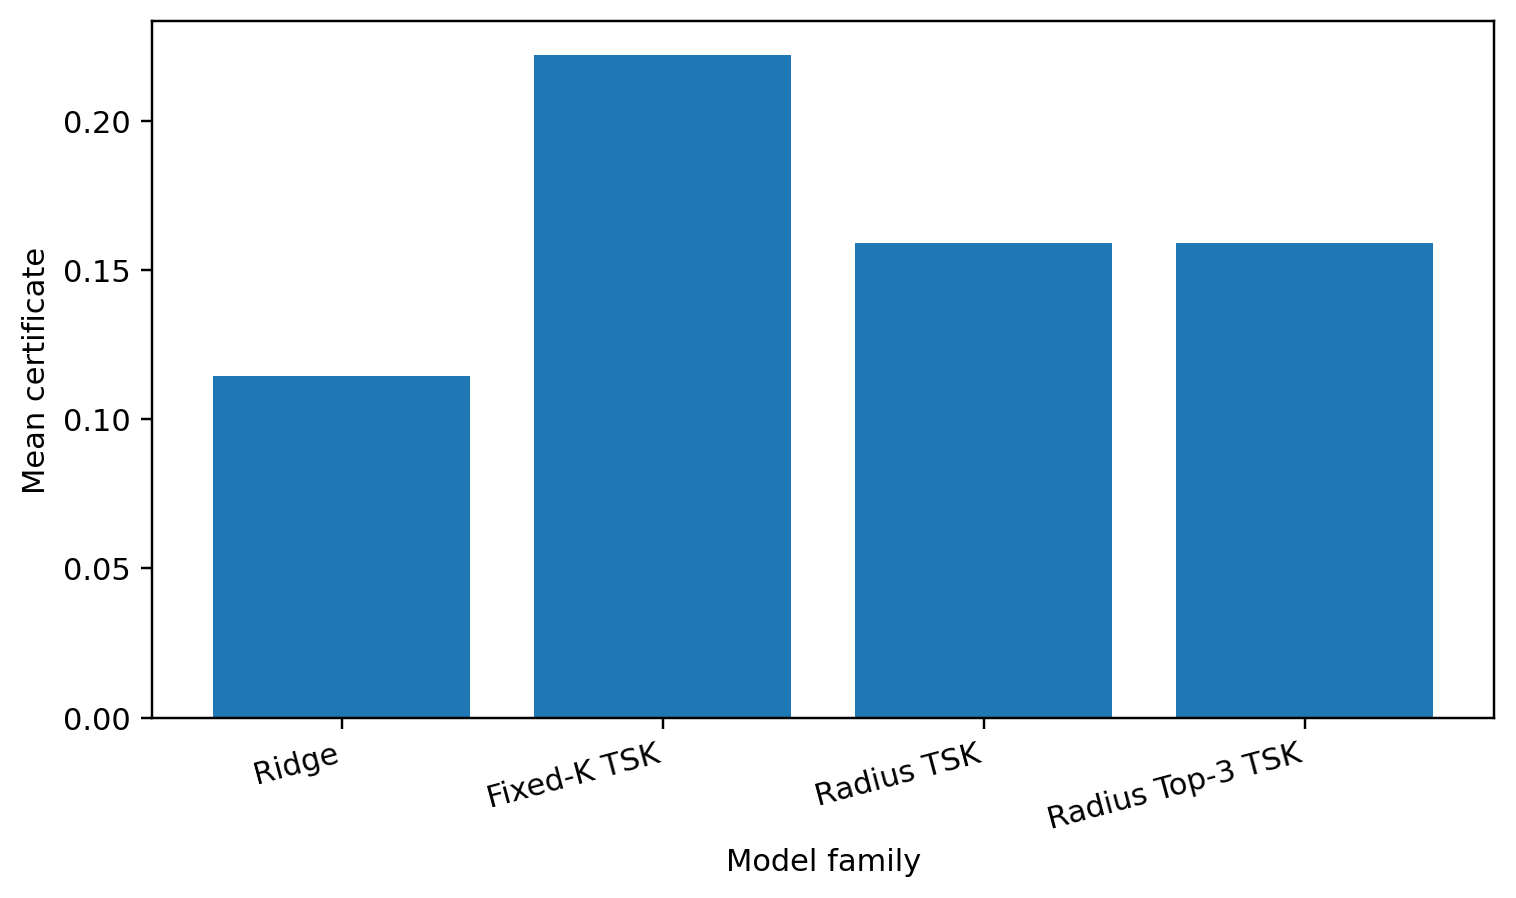
\includegraphics[width=\columnwidth]{figures/structural_certificate_by_family.png}
\caption{Mean familywise certificate under validation-RMSE selection across 30 synthetic development series. Ridge is tightest; radius control substantially improves on the originally prespecified fixed $K=12$ TSK baseline.}
\label{fig:structural_cert}
\end{figure}


\subsection{Fixed-$K$ Sensitivity Qualifies the Radius Advantage}
\begin{table}[t]
\caption{Fixed-$K$ sensitivity under validation-RMSE selection across 30 synthetic development series. The paired difference is Radius TSK minus Fixed-$K$ TSK; negative values favor radius control.}
\label{tab:fixed_k_sensitivity}
\centering
\footnotesize
\begin{tabular}{rrrrrr}
\toprule
$K$ & Dimension & Gaussian KL & Certificate & Test RMSE & $\Delta$ Cert. \\
\midrule
2 & 23.7 & 10.180 & 0.1326 & 0.8850 & +0.0264 \\
3 & 34.3 & 13.469 & 0.1465 & 0.8846 & +0.0125 \\
4 & 41.9 & 17.294 & 0.1568 & 0.8869 & +0.0021 \\
6 & 60.0 & 21.011 & 0.1701 & 0.8950 & -0.0112 \\
8 & 82.9 & 26.413 & 0.1875 & 0.8951 & -0.0286 \\
12 & 135.6 & 39.547 & 0.2221 & 0.9149 & -0.0631 \\
\bottomrule
\end{tabular}
\end{table}


Table~\ref{tab:fixed_k_sensitivity} shows that the mean fixed-$K$ certificate increases steadily with rule count, from 0.1326 at $K=2$ to 0.2221 at $K=12$. The radius-controlled mean is 0.1589. Consequently, radius control is not uniformly tighter than fixed rule bases: its mean certificate is looser than fixed $K=2$ and $K=3$, essentially matched by $K=4$, and tighter than the larger $K=6,8,12$ alternatives. After Holm correction, the paired certificate advantage is clear for $K=8$ and $K=12$, while the differences for $K=3,4,6$ are not statistically decisive.

When each series is allowed to choose its best fixed $K$ by validation RMSE, radius control changes the certificate by only $-0.0068$ on average (radius minus best fixed $K$; 95\% bootstrap interval $[-0.0187,0.0049]$) and the paired Wilcoxon result is not significant after correction. The corresponding test-RMSE difference is $-0.0054$ with bootstrap interval $[-0.0118,-0.0002]$, but the rank test is again not significant after multiplicity correction. Nine of 30 series select $K=2$, five select $K=3$, four select $K=4$, six select $K=6$, five select $K=8$, and only one selects $K=12$. Under certificate selection, all 30 series select fixed $K=2$.

These results materially narrow the structural claim. Radius construction is useful as an adaptive mechanism that avoids large unnecessary rule bases, but the certificate gain relative to $K=12$ is mainly a rule-count effect. The current evidence does not show that radius control dominates a predeclared and fairly charged small fixed-$K$ grid.

\begin{figure}[t]
\centering
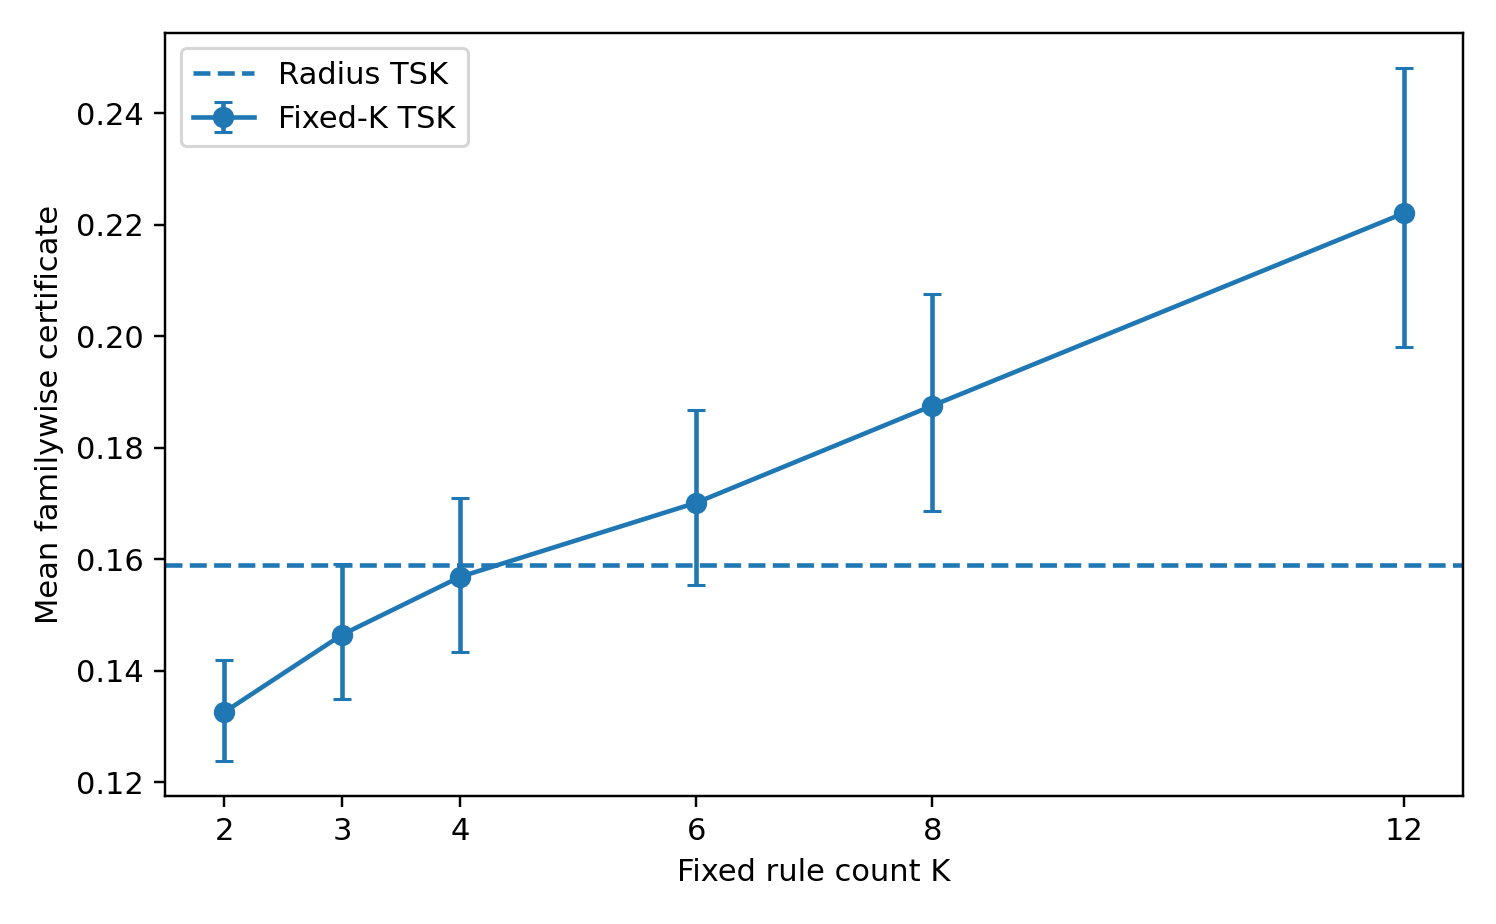
\includegraphics[width=\columnwidth]{figures/fixed_k_certificate_sensitivity.png}
\caption{Mean familywise certificate for fixed-$K$ TSK under validation-RMSE selection. Error bars are bootstrap intervals for the per-series means; the dashed line is the radius-controlled TSK mean.}
\label{fig:fixed_k_sensitivity}
\end{figure}

\begin{figure}[t]
\centering
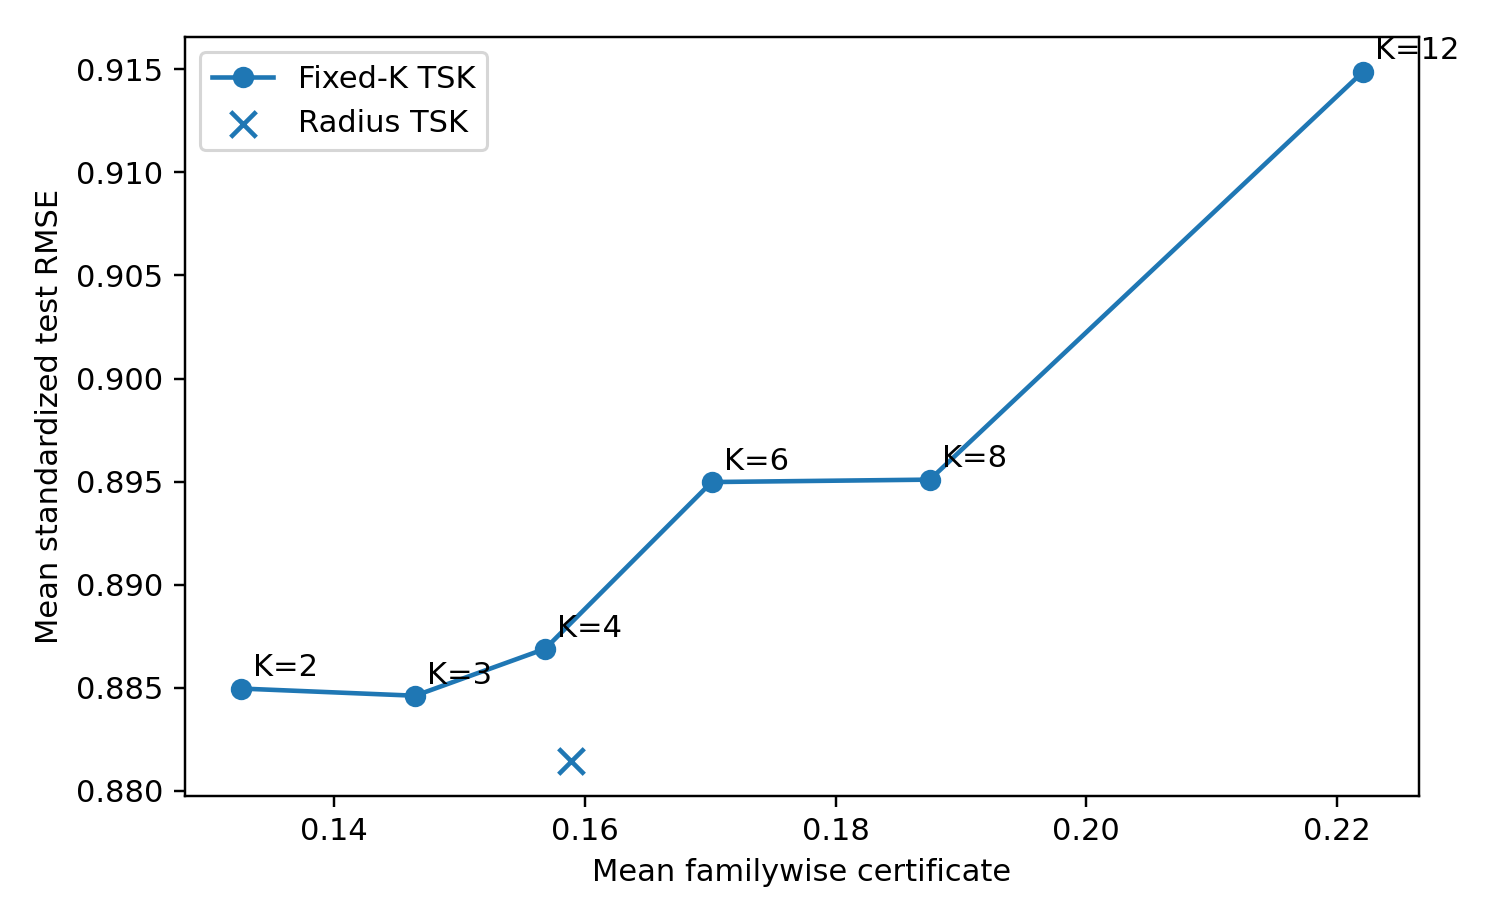
\includegraphics[width=\columnwidth]{figures/fixed_k_pareto_sensitivity.png}
\caption{Development mean test RMSE versus mean familywise certificate across fixed rule counts and radius-controlled TSK. The plot is descriptive and does not imply a universal Pareto ordering.}
\label{fig:fixed_k_pareto}
\end{figure}

\subsection{The Radius--Rule--Dimension--KL Chain}
Within each process, family, and lag, Spearman correlations across radius values average $-0.847$ for radius versus rule count, $1.000$ for rule count versus dimension, $0.981$ for dimension versus Gaussian KL, and $0.982$ for Gaussian KL versus certificate. These are descriptive associations rather than a universal monotonicity theorem, but they make the realized complexity path observable:
\begin{equation}
r\longrightarrow K(r)\longrightarrow D(r)\longrightarrow \mathrm{KL}\longrightarrow \operatorname{Cert}.
\end{equation}

Ridge retains the smallest mean certificate under both selection strategies: 0.1145 under validation-RMSE selection and 0.1017 under certificate selection. The results therefore do not support a claim that TSK is intrinsically easier to certify than a linear model.

\subsection{Predictive Accuracy and Clipping}
\begin{table*}[t]
\centering
\caption{Synthetic development results selected by validation RMSE (five seeds per process). RMSE is on the prior-standardized scale.}
\label{tab:process_results}
\small
\setlength{\tabcolsep}{5pt}
\begin{tabular}{lrrrrrr}
\toprule
& \multicolumn{2}{c}{Test RMSE} & \multicolumn{2}{c}{Certificate} & \multicolumn{2}{c}{Target clipping} \\
\cmidrule(lr){2-3}\cmidrule(lr){4-5}\cmidrule(lr){6-7}
Process & Ridge & Radius TSK & Ridge & Radius TSK & Cert. & Test \\
\midrule
AR(2) & 0.9098 & 0.9126 & 0.1128 & 0.1271 & 0.62\% & 0.35\% \\
SETAR & 1.0140 & 0.9798 & 0.1131 & 0.1467 & 0.42\% & 0.50\% \\
NARMA-10 & 0.7670 & 0.7656 & 0.1093 & 0.1188 & 0.97\% & 0.30\% \\
Mackey--Glass & 0.0656 & 0.0539 & 0.1129 & 0.2403 & 0.92\% & 1.30\% \\
GARCH & 1.0398 & 1.0926 & 0.0941 & 0.1114 & 0.25\% & 0.20\% \\
Structural break & 1.5236 & 1.4841 & 0.1445 & 0.2093 & 23.87\% & 71.55\% \\
\bottomrule
\end{tabular}
\end{table*}


Table~\ref{tab:process_results} separates predictive accuracy from certificate tightness. Radius TSK improves mean test RMSE over ridge on SETAR, NARMA-10, Mackey--Glass, and the structural-break process, but is slightly worse on AR(2) and materially worse on GARCH. Its largest benefit is Mackey--Glass, where mean RMSE falls from 0.0656 to 0.0539, while its certificate is more than twice the ridge value because of additional complexity.

The structural-break process is a failure-boundary example. Certification target clipping is 23.87\% and test target clipping is 71.55\%. The bounded certificate remains formally meaningful for the clipped loss, but it is not an operational description of raw errors after the break.

The localized prior improves the selected familywise certificate over a zero-mean prior in 85.6\% of selected rows, with mean absolute improvement 0.0138 after charging the same prior-variant mixture cost. Localization is useful but not uniformly superior; GARCH contains counterexamples.

\subsection{Negative Tetouan Development Outcome}
The initial Tetouan gate admits a radius TSK model in zone 1 and a fixed-$K$ TSK model in zone 2, while zone 3 abstains. Both learned deployments fail on the test horizon: RMSE changes are $-11.86\%$ and $-1.51\%$, and asymmetric-cost changes are $-22.67\%$ and $-19.05\%$. Averaged over all three zones, including the zone-3 fallback, RMSE worsens by 4.46\% and cost worsens by 13.91\%.

This negative result demonstrates that a non-vacuous certificate plus overall validation performance is not a sufficient deployment rule under temporal shift. It motivated the stricter margin and block-stability requirements in the independent confirmatory protocol.

\subsection{Independent PJM Confirmatory Outcome}
\begin{table*}[t]
\centering
\caption{Operational decision studies. Improvements are relative to the predeclared seasonal-naive fallback; negative values indicate degradation.}
\label{tab:energy_decisions}
\small
\setlength{\tabcolsep}{4pt}
\begin{tabular}{lllr rr}
\toprule
Phase & Series & Deployment & Certificate & Test RMSE imp. & Test cost imp. \\
\midrule
Tetouan dev. & zone 1 & dense\_tsk & 0.1226 & -11.86\% & -22.67\% \\
Tetouan dev. & zone 2 & fixed\_k\_dense\_tsk & 0.1482 & -1.51\% & -19.05\% \\
Tetouan dev. & zone 3 & seasonal\_naive\_24h & -- & 0.00\% & 0.00\% \\
\midrule
PJM confirm. & AEP & ridge & 0.0959 & 57.97\% & 58.64\% \\
PJM confirm. & COMED & ridge & 0.0841 & 55.40\% & 54.11\% \\
PJM confirm. & DAYTON & dense\_tsk & 0.0933 & 49.13\% & 50.30\% \\
PJM confirm. & PJME & ridge & 0.0959 & 51.70\% & 51.42\% \\
\bottomrule
\end{tabular}
\end{table*}


The frozen PJM gate admits a learned model in all four regions. Test RMSE improves by 57.97\%, 55.40\%, 49.13\%, and 51.70\% for AEP, COMED, DAYTON, and PJME, respectively. Corresponding asymmetric-cost improvements are 58.64\%, 54.11\%, 50.30\%, and 51.42\%; mean improvements are 53.55\% and 53.62\%. Selected certificates range from 0.0841 to 0.0959, and test target and forecast clipping are zero.

\begin{figure}[t]
\centering

\includegraphics[width=\columnwidth]{figures/pjm_test_improvements.png}
\caption{Independent PJM test improvements over the frozen seven-day seasonal-naive fallback.}
\label{fig:pjm_improvements}
\end{figure}

The confirmatory result does not establish nonlinear fuzzy superiority. AEP, COMED, and PJME select ridge. DAYTON selects a radius-controlled one-rule TSK with lag 14; with one rule, this is an affine predictor. No fixed-eight-rule TSK candidate passes the frozen gate. The operational evidence therefore supports a complexity-aware gate that can shrink to a simple model, not a claim that a multi-rule TSK system caused the gain.

\section{Discussion and Limitations}
\label{sec:discussion}

\subsection{What the Evidence Supports}
The structural ablation supports a narrower claim than the original $K=12$ contrast alone suggested. Replacing an unnecessarily dense fixed rule base by a prior-only radius cover reduces the realized rule count, randomized dimension, Gaussian KL, and certificate. However, the multi-$K$ sensitivity shows that small fixed rule bases can match or improve on the radius-controlled certificate. Thus the robust conclusion is that true rule-block reduction matters, not that radius construction is intrinsically superior to every fixed-$K$ design. This effect remains distinct from Top-3 activation, which leaves the randomized parameter space unchanged.

The operational studies support a second, different claim. A certificate can be used as one eligibility condition in a decision rule, but it must be combined with a meaningful baseline margin and temporal-stability checks. The failed Tetouan gate and successful frozen PJM gate are both part of the evidence. Hiding the negative development case would make the confirmatory result appear stronger than the protocol justifies.

\subsection{What the Evidence Does Not Support}
First, ridge has the tightest average certificate, so the study does not show that fuzzy models are generally more certifiable. Second, the PJM decisions are linear or one-rule affine models; the real-data case does not demonstrate a practical advantage from nonlinear multi-rule fuzzy partitioning. Third, the PJM comparison is against a predeclared seven-day seasonal-naive fallback, not SARIMA, gradient boosting, or deep forecasting systems. The 49--58\% improvements should not be generalized beyond that comparison.

Fourth, the certificate is not a raw-RMSE guarantee. The conditional sequential risk in Proposition~\ref{prop:bound} belongs to the clipped Gibbs/BMA predictor over the certification horizon. The independent test horizon is used only for empirical confirmation of the frozen deployment decision. Future deployment under a new shift would require a new online or rolling protocol.

\subsection{Remaining Methodological Limitations}
The synthetic ablation contains five seeds per process, sufficient to expose large structural effects but not to characterize every nonlinear regime. The strong structural-break process shows that a prior-fixed clipping interval can lose operational meaning. Heavy-tail or variance-adaptive supermartingale bounds \cite{haddouche2023heavy,rodriguez2024more} are a principled next direction, but they require a separate verified implementation.

The time-uniform proposition is evaluated numerically only at the final certification horizon. We do not claim an executed confidence sequence over all prefixes. The hierarchical prior is finite and auditable, but its fixed grids constrain the model family. The PJM study contains only four regional series and one common historical interval. Finally, infrastructure interrupted the first confirmatory invocation before test opening; the restart used unchanged hashes and is fully disclosed, but an uninterrupted run would be procedurally cleaner.

\subsection{Implications for Fuzzy-System Design}
The main design implication is that interpretability-oriented rule reduction and PAC-Bayesian complexity can align when sparsity removes complete rule blocks. Pruning only the active firing strengths is not enough if every consequent remains randomized and charged. A future certificate-aware TSK learner should therefore optimize a true structural posterior over rule inclusion, rather than relying only on sparse activation at prediction time. Such a method could make the fuzzy contribution stronger than the current deterministic radius construction.

\section{Conclusion}
\label{sec:conclusion}

We presented an audited, chronological specialization of a known time-uniform PAC-Bayes supermartingale bound for ridge and TSK time-series predictors. The complete model index includes the ridge penalty and all structural choices, and the certified loss is explicitly clipped and normalized. A controlled development ablation shows that radius-controlled rule-count sparsity substantially reduces randomized dimension, KL, and certificate value relative to a dense 12-rule TSK structure, whereas Top-3 activation alone does not. A subsequent multi-$K$ sensitivity analysis qualifies this result: small fixed rule bases can match or tighten the radius-controlled certificate, so the supported mechanism is removal of complete rule blocks rather than a universal advantage of radius selection. Ridge nevertheless remains the easiest family to certify on average.

The real decision studies provide a complementary result. A permissive Tetouan gate failed, while a redesigned gate frozen before an independent PJM study improved both RMSE and asymmetric cost in all four regions relative to the predeclared seasonal fallback. Because the selected models were ridge or one-rule TSK, this is evidence for complexity-aware selection and abstention rather than fuzzy-model dominance.

The defensible conclusion is therefore limited but useful: structural rule reduction can tighten a PAC-Bayesian certificate, and a certificate can contribute to an operational gate when it is not confused with a direct performance guarantee. Future work should develop posterior rule selection, compare against stronger operational baselines, and replace clipping with verified heavy-tail or variance-adaptive sequential bounds.


\section*{Data and Code Availability}
The complete code, frozen configurations, raw result tables, pre-outcome locks, and audit manifests are included in the accompanying reproducibility artifact. The public repository URL will be inserted in the final submission; the review package uses an anonymized archive.

\bibliographystyle{IEEEtran}
\bibliography{refs}

\end{document}
